%**************************************************************************
%* SpringSim 2020 Author Kit
%*
%* Word Processing System: TeXnicCenter and MiKTeX
%*
%**************************************************************************

\documentclass{scspaperproc}

\usepackage{latexsym}
\usepackage{graphicx}
\usepackage{mathptmx}

%
%****************************************************************************
% AUTHOR: You may want to use some of these packages. (Optional)
\usepackage{amsmath}
\usepackage{amsfonts}
\usepackage{amssymb}
\usepackage{amsbsy}
\usepackage{amsthm}
%****************************************************************************

%
%****************************************************************************
% AUTHOR: If you do not wish to use hyperlinks, then just comment
% out the hyperref usepackage commands below.

%% This version of the command is used if you use pdflatex. In this case you
%% cannot use ps or eps files for graphics, but pdf, jpeg, png etc are fine.

\usepackage[pdftex,colorlinks=true,urlcolor=blue,citecolor=black,anchorcolor=black,linkcolor=black,bookmarks=false]{hyperref}

%% The next versions of the hyperref command are used if you adopt the
%% outdated latex-dvips-ps2pdf route in generating your pdf file. In
%% this case you can use ps or eps files for graphics, but not pdf, jpeg, png etc.
%% However, the final pdf file should embed all fonts required which means that you have to use file
%% formats which can embed fonts. Please note that the final PDF file will not be generated on your computer!
%% If you are using WinEdt or PCTeX, then use the following. If you are using
%% Y&Y TeX then replace "dvips" with "dvipsone"

%% \usepackage[dvips,colorlinks=true,urlcolor=blue,citecolor=black,%
%% anchorcolor=black,linkcolor=black]{hyperref}

%% The use of the long citation format (e.g. "Brown and Edwards (1993)" rather than "[5]") and at the same
%% time using the hyperref package can lead to hard to trace bugs in case the citation is broken accross the
%% line (usually this will mark the entire paragraph as a hyperlink (clickable) which is easily noticeable and fixed
%% if using colorlinks, but not if the color is black -- as it is now). Worse yet, if a citation spans page boundary,
%% LaTeX compilation can fail, with an obscure error message. Since this depends a lot on the flow of the text
%% and wording, these bugs come and go and can be extremely hard for a beginner to trace. The error
%% message can look like this:
%%
%%    ! pdfTeX error (ext4): \pdfendlink ended up in different nesting level than \pdfstartlink.
%%    \AtBegShi@Output ...ipout \box \AtBeginShipoutBox 
%%    \fi \fi 
%%    l.174 
%%    ! ==> Fatal error occurred, no output PDF file produced!
%%
%% and can be universally fixed by putting an \mbox{} around the citation in question (in this case, at line 174)
%% and maybe adapting the wording a little bit to improve the paragraph typesetting, which is perhaps not
%% immediately obvious.
%****************************************************************************

%****************************************************************************
%*
%* AUTHOR: YOUR CALL!  Document-specific macros can come here.
%*
%****************************************************************************

%% Command for creating multiplie-line cells inside a table environment
\newcommand{\multiline}[2][c]{{%
  \begin{tabular}%
    [#1]{@{}c@{}}#2%
  \end{tabular}%
}}

%% Use a package to allow for multi-row cells in a table.
\usepackage{multirow}

% add custom hyphenation rules here
\usepackage{hyphenat}
\hyphenation{op-tical net-works semi-conduc-tor}

% If you use theorems
\newtheoremstyle{scsthe}% hnamei
{8pt}% hSpace abovei
{8pt}% hSpace belowi
{\it}% hBody fonti
{}% hIndent amounti1
{\bf}% hTheorem head fontbf
{.}% hPunctuation after theorem headi
{.5em}% hSpace after theorem headi2
{}% hTheorem head spec (can be left empty, meaning `normal')i

\theoremstyle{scsthe}
\newtheorem{theorem}{Theorem}
\renewcommand{\thetheorem}{\arabic{theorem}}
\newtheorem{corollary}[theorem]{Corollary}
\renewcommand{\thecorollary}{\arabic{corollary}}
\newtheorem{definition}{Definition}
\renewcommand{\thedefinition}{\arabic{definition}}

% avoid overrunning the right margin; you are welcome to remove this, provided that you take care not to overrun the right margin anywhere in your paper
\sloppy

%#########################################################
%*
%*  The Document.
%*
\begin{document}

%***************************************************************************
% AUTHOR: Thomas C.H. Lux and Tyler H. Chang
% FORMAT AUTHORS NAMES Like: Author1, Author2 and Author3 (last names)
%
%		You need to change the author listing below!
%               Please list ALL authors using last name only, separate by a comma except
%               for the last author, separate with "and"


\SCSpagesetup{Lux and Chang}

% AUTHOR: Uncomment ONE of these correct conference names.
\def\SCSconferenceacro{SpringSim'20}
%\def\SCSconferenceacro{SummerSim}
%\def\SCSconferenceacro{AutumnSim}
%\def\SCSconferenceacro{PowerPlantSim}

% AUTHOR: Set the correct year of the conference.
\def\SCSpublicationyear{2020}

% AUTHOR: Set the correct month and dates; the dates are separated by a single minus sign
% with no spaces and no leading zeros, the month is a full name (e.g. April) with the first letter
% capitalized. For example, "April 8-13".
\def\SCSconferencedates{May 19-May 21}

% AUTHOR: Set the correct venue in the form "City, State, Country", for example "Los Angeles, CA, USA".
\def\SCSconferencevenue{Fairfax, VA, USA}

% AUTHOR: Enter the title, all letters in upper case
\title{Metric Principle Component Analysis: \\ On Identifying Important Subspaces for Approximation}

% AUTHOR: Enter the authors of the article, see end of the example document for further examples
\author{
Thomas C. H. Lux\\
Tyler H. Chang\\ [12pt]
Department of Computer Science\\
Virginia Polytechnic Institute \& State University\\
2000 Torgersen Hall, Blacksburg, VA, USA\\
\{tchlux,thchang\}@vt.edu\\
}


\maketitle

%% Examples and notes.
%% 
%% \begin{table}[htb]
%%   \centering
%%   \caption{Caption above the table!}\label{tab:example}
%%   \begin{tabular}{r|l}
%%     First & row \\ \hline
%%     second & row \\
%%     third & row \\
%%   \end{tabular}
%% \end{table}
%% 
%% \begin{figure}[htb]
%%   \centering
%%   \includegraphics[width=0.50\textwidth]{path_without_extension}
%%   \caption{Caption below the figure!}\label{fig:example}
%% \end{figure}
%% 
%% \cite{ref}  - Make a citation that is in parenthesis
%% \citeN{ref} - Make a citation out of parenthesis (for noun usage)
%% \shortcite{ref}  - Make a citation for references with >3 authors.
%% \shortciteN{ref} - Make a noun-form citation for references with >3 authors.
%% 
%% 
%% 5 - 12 page paper mandated
%% 150 word abstract
%% 5 keywords maximum


\section*{Abstract}

Many modern data science problems for approximation have high
dimension while the true underlying phenomenon can be accurately
represented from a fraction of the provided information. A variety of
dimension reduction techniques exist, but most target unsupervised
applications rather than approximation problems or only accommodate a
small set of approximation problems. This paper presents metric
principle component analysis (MPCA), an extension of standard
principle component analysis (PCA) that accounts for metric variation
in applied approximation problems like classification and
regression. MPCA is theoretically motivated, shown to be a superset of
classical PCA, and its usefulness as a dimension reduction technique
for approximation problems is demonstrated. Initial results reveal
both that MPCA can be significantly better in some cases, and that in
other applications it performs similarly to standard PCA.

\textbf{Keywords:} principle component analysis, classification,
regression, approximation, metric learning


\section{Introduction}
\label{sec:introduction}

Dimension reduction is an important problem in data science and, more
generally, function approximation. Consider a multivariable function
$f : \mathbb{R}^d \rightarrow (S, m)$ where $(S,m)$ denotes a metric
space with metric $m$. In the context of data science, $(S,m)$ could
represent a discrete classification space, a continuous real-valued
space, or could be descriptive of some graph structure. In this paper,
the supervised learning problem is considered, where a finite set $X
\subset \mathbb{R}^d$ of data points are given along with labeled
function values $Y = \{y_i = f(x_i) | x_i \in X\}$.  There are many
algorithms in the field of data science, mathematics, and machine
learning for predicting general functions such as multivariate spline
approximations, neural networks, clustering algorithms, support vector
machines/regressors, and more. One particularly common yet effective
class of solutions to these problems are distance based approximations
such as k-nearest neighbor (KNN).  Though effective for many classes
of problems, these methods depend on the premise that distance in the
input space can be associated with change in the output class or
value. While this assumption holds for most of the common "big data"
problems, it is often the case that some number of directions in the
input space have no bearing on the output class/value. Without
applying dimension reduction, these directions will increase the cost
of any distance based approximation techniques, in some cases making
the prediction techniques computationally intractable.  Furthermore,
such "meaningless directions" cannot improve prediction accuracy, and
often decrease accuracy by disassociating distance from change in
class/value.

In this paper, a novel technique for performing dimension reduction is
proposed that considers how the output $f(x)$ changes given the data
$X$ and function value/labels $Y$. Using this information, an
orthonormal basis is constructed for a new subspace of $\mathbb{R}^d$
where every direction is associated with some change in $f$, thereby
increasing the accuracy of distance based methods while often
significantly reducing the dimension. The technique is model agnostic,
meaning that it can be applied as a "pre-conditioning" step before any
distance based approximation. The effectiveness of the technique is
demonstrated on one theoretical and three real-world problems, using
four different distance based approximation algorithms as well as a
multi-layer perceptron (MLP).

The remainder of this paper is structured as follows: Section
\ref{sec:background} considers existing dimension reduction techniques
for approximation problems, Section \ref{sec:methodology} explains the
methodology of computing MPCA and provides a theoretical example,
Section \ref{sec:results} shows results on real-world problems,
Section \ref{sec:discussion} discusses the implications of results,
and finally Section \ref{sec:conclusion} concludes.


\section{Background}
\label{sec:background}

\subsection{Related Work}
\label{sec:related}

One of the most standard methods for performing dimension reduction is
correlation analysis, whereby a general model\footnote{The model may be a
multivariable linear or quadratic model, possibly with interaction
terms.} is fit\footnote{Most commonly fits are performed via least-squares
approximation.} to the data and the coefficients of each term are
analyzed to determine whether that term has any effect on the
output. After dropping all terms that have no statistically
significant effect on the function value, it can be inferred that only
the directions associated with the remaining terms affect the output
class or function value. These techniques are highly effective when an
appropriate model is chosen, but are highly model dependent and
generally fail for a black-box output function $f$. For example, this
technique is most commonly applied by fitting a linear model to
labeled data. Then, if the function $f$ is not itself approximately
linear, the above technique can fail to produce any meaningful
results.

Principle component analysis (PCA) is another commonly used dimension
reduction technique. An explanation of Principle Component Analysis
and its applications can be found in
\citeN{PCAtutorial,powell_lehe_2014}. Given a finite set of unlabeled
points $X \subset \mathbb{R}^d$, PCA identifies an ordered set of
orthonormal basis vectors $\{v_1, \ldots, v_d\},$ such that the
projection of $X$ onto any subspace defined by the span of $\{v_1,
\ldots, v_k\},$ $k \leq d$ has maximal variance. Equivalently, PCA is
the dimension reduction technique that minimizes reconstruction error
for $X$ with respect to mean squared error (MSE). In its standard
application, PCA is an unsupervised technique, and does not consider
the effect of each dimension on output class or function values.

Recently a modified variant of PCA was proposed which incorporates
function values into the subspace basis and the technique is referred
to as \textit{supervised PCA}
\shortcite{barshan2011supervised}. However this technique relies on
the coefficients of a linear fit and faces the same nonlinear
approximation weaknesses (as will be demonstrated in a theoretical
example).

Other notable techniques include linear discriminant analysis (LDA)
and neural network autoencoders. LDA depends heavily on linear
separability of the output classes, and therefore can fail for a
general function $f$. In their most naive implementation, autoencoders
are equivalent to standard PCA. However, they can be modified to also
consider output labels, though no convergence guarantees can be made
and the results are purely heuristic. Other feature weighting
techniques have been studied for clustering and generic learning
algorithms
\shortcite{FeatureWeightingForClustering,FeatureWeightingReview}, and
in general a lot of work has been done on feature selection given a
model \shortcite{FeatureSurvey,tenenbaum2000global}. Those survey
papers extensively cover existing techniques and approaches for
weighting (continuous valued) and selecting (binary operation)
features of data for making accurate approximations.

\subsection{Approximation Techniques}
\label{sec:approximation}

Four distance based approximation techniques are used to validate the
proposed dimension reduction technique and additionally a classic
neural network is tested. The first approximation algorithm is
k-nearest neighbor using the 2-norm distance with $k=1,$ and the
second is the same method with $k=10.$ By sorting points in a tree,
k-nearest neighbors is able to scale linearly with the input dimension
and near logarithmically with respect to number of input points. The
second technique is the modified linear Shepard's method called LSHEP
\shortcite{thacker2010algorithm}. LSHEP incorporates a local linear
fit into the the original Shepard's method \shortcite{shepard1968two},
an inverse distance weighting technique that scales linearly with
dimension and linearly with number of points. The final distance based
technique uses the Delaunay triangulation, a piecewise linear
interpolant based on a simplicial mesh of the same name
\shortcite{chang2018polynomial}. Of the above techniques, Delaunay is
the most computationally expensive, scaling approximately linearly
with number of points, but growing prohibitively expensive in
dimension greater than 50. The last technique for general comparison
is a classic neural network called a Multi-Layer Perceptron
(MLP). This work uses the implementation available at
\shortcite{scikit-learn} while choosing the Rectified Linear Unit
(ReLU) activation function and Stochastic Gradient Descent (SGD) error
minimizer. 1000 gradient steps are allowed to be taken and the default
number of hidden nodes (100) is used with one hidden layer.


\section{Methodology}
\label{sec:methodology}

In this section, a novel application of Principle Component Analysis
(PCA) is proposed in order to perform dimension reduction in a
supervised learning (approximation) context. The method will be
referred to as Metric PCA (MPCA).

Let $f : \mathbb{R}^d \rightarrow (S,m)$ be an arbitrary function of
interest, where $(S,m)$ is a metric space and $d$ is a positive
integer.  Let $X \subset \mathbb{R}^d$ be a finite set of points with
known function values (labels) $Y = \{y_i = f(x_i) | x_i \in X\}$.
Consider the set $Z$ of vectors

\begin{equation*}
  Z = \bigg\{ \frac{(x_i - x_j)\  m(y_i, y_j)}{\|(x_i - x_j)\|_2^2} : \quad x_i, x_j \in X, \quad y_i, y_j \in Y \bigg\},
\end{equation*}

\noindent with covariance matrix $Cov(Z).$ Note that since $Cov(Z)$ is
symmetric, its Eigenvectors are orthogonal and form a basis for
$\mathbb{R}^d$. Note that if the original set $X$ contains
$n$ points, then the new set $Z$ must contain $\mathcal{O}(n^2)$
points, since it consists of all vectors \textit{between} points in $X$,
rescaled by change in their corresponding function values (in $Y$).

An Eigenvector decomposition is performed on $Cov(Z),$ then the points
are reduced into the lower-dimensional space spanned by the first $k$
Eigenvectors ranked by the magnitude of their corresponding
Eigenvalues (i.e., PCA on the new set $Z$). A \textit{magnitude} is
assigned to each vector by computing the \textit{total variation} of
the function along each Eigenvector and normalizing the sum of
magnitudes to be one. In practice, instead of performing an
Eigenvector decomposition on $Cov(Z),$ a singular value decomposition
is performed on the matrix $\displaystyle Z^\star$, whose rows are
transposed vectors in $Z$. Then, $Z^\star = U \Sigma V^T$, and the
columns of $V$ are exactly the Eigenvectors of $Cov(Z).$

\subsection{Equivalence of PCA and MPCA Under Euclidean Distance Metric}

In this section it is shown that in the special case where $m(y_i,y_j)
= \|x_i - x_j\|_2$, MPCA is identical to PCA.

Given $X$ as stated above, if the set of all pairwise difference
vectors $Z$ is considered, then $PCA(Z) = PCA(X).$ Denote $Z_j$ to be
the subset of $Z$ about vertex $x_j \in X,$ $Z_j = \{x_j - x_i : x_i
\in X\}.$ Consider the first principle component of $X,$ $v_1 \in
\mathbb{R}^d.$ It is noted that the first principle component of $Z$
is the same, and will follow that all remaining components are
identical.

\begin{align*}
  \max_{\|v\|_2 = 1} \|Zv\|_2^2
  =& \max_{\|v\|_2 = 1} \sum_{z \in Z} \langle z, v \rangle^2
  = \max_{\|v\|_2 = 1} \sum_{Z_j \subset Z} \sum_{z \in Z_j} \langle z, v \rangle^2 \\
  \leq&\ \sum_{Z_j \subset Z} \max_{\|v\|_2 = 1} \sum_{z \in Z_j} \langle z, v \rangle^2 
  = \ \sum_{Z_j \subset Z} \sum_{z \in Z_j} \langle z, v_1 \rangle^2 \\
  =& \sum_{z \in Z} \langle z, v_1 \rangle^2 
  = \ \|Zv_1\|_2^2 \\
  \implies&\max_{\|v\|_2 = 1} \|Zv\|_2 = \|Zv_1\|_2.
\end{align*}

After removing the first component from each vector in $Z$, the same
technique can be reapplied to find the second component. This
methdology can be applied to the remaining components in an inductive
fashion, to show total equivalence of the principle components for $X$
and $Z.$

\begin{figure}
  \centering
  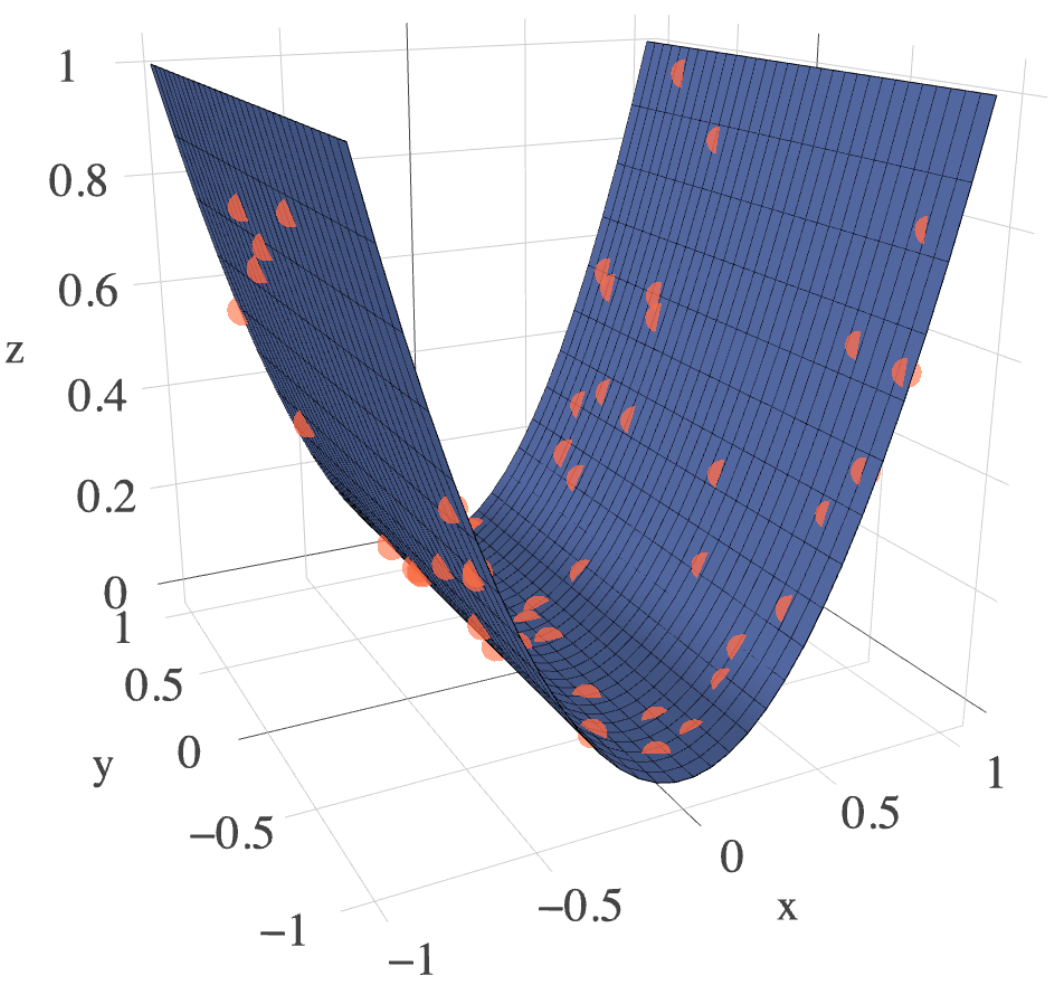
\includegraphics[width=0.30\textwidth]{1-mpca-pca.png}
  \hspace{5mm}
  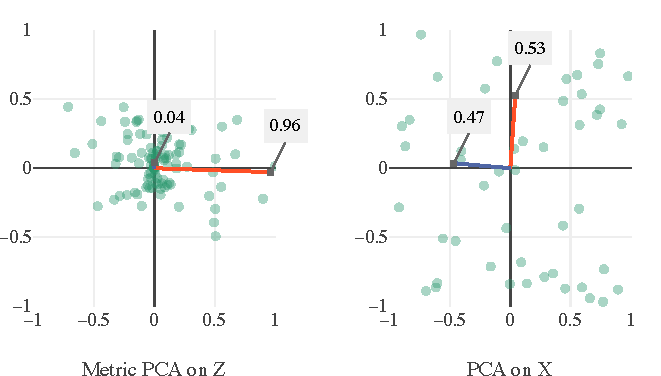
\includegraphics[width=0.53\textwidth]{1-mpca-pca.pdf}
  \caption{Depicted above from left to right are source data for an
    approximation problem (red dots, on left) and a true underlying
    function (blue mesh, on left), the constructed point set $Z$ with
    metric principle components (middle), and the source point set $X$
    with standard principle components (right). Notice that the MPCA
    components are ordered and weighted in proportion to their
    relevance to the true function, while the PCA components are
    unrelated to the underlying function.}
  \label{fig:analytic}
  %% {{https://people.cs.vt.edu/tchlux/files/[2018-11-28]_mpca_demo_2.html}}
\end{figure}


\subsection{Analytic Demonstration}

Consider the following example. In this, $X^{(50\ \times\ 2)}$ is a
random sample of points drawn from the unit cube and the values come
from a function $f: \mathbb{R}^2 \rightarrow \mathbb{R},$ defined as
$f(x,y) = x^2$ and note that this only depends on the $x$
direction. The results of applying PCA and MPCA to this problem can be
seen in Figure \ref{fig:analytic}. It is clear that the example set of
points are not distributed according the direction of greatest change
in the underlying function. This causes PCA to produce distinctly
different vectors from MPCA, noting that the standard principle
components are not only irrelevant to approximation, they are ordered
incorrectly in terms of importance. It should be noted that this
symmetric underlying function would cause \textit{supervised PCA} to
fail, since no meaningful linear fit can be produced.


\begin{table}
  \centering
  \renewcommand{\arraystretch}{1.2}
  \begin{tabular}{l l}
    \hline
    \textit{Methods} & PCA, MPCA \\
    \hline
    \textit{Approximators} & KNN (1), KNN (10), LSHEP, Delaunay, MLP \\
    \hline
    \textit{Number of samples (for MPCA)} & n, 10n \\
    \hline
    \textit{Fraction of original dimension (for reduction)} & $1/3$, $1/10$, $1/100$ \\
    \hline
  \end{tabular}
  \vspace{5mm}
  \caption{All possible combinations of the above settings are
    considered in experiments. Four distance based techniques are
    tested as well as a classical neural network. Since MPCA requires
    the construction of a pairwise difference set of points, random
    samples of size $n$ and $10n$ are drawn to prevent drastic
    increase in the amount of data.}
  \label{tab:evaluation}
\end{table}

\subsection{Evaluation}

Given theoretical interest in MPCA, it is important to evaluate the
performance of MPCA by applying it to real approximation problems. In
this section, MPCA is applied to three such real problems, two image
classification problems (MNIST, CIFAR10) and one regression problem
(Yelp rating prediction). First, the performance of four common
approximation algorithms applied to the raw training data is evaluated
using four-fold cross validation. Then, the dimension is reduced to
various percentages of the total dimension using both MPCA and PCA and
the performance of each algorithm is reevaluated. Recall that when $X$
contains $n$ data points, the transformed set $Z$ contains
$\mathcal{O}(n^2)$ points. Therefore, MPCA requires the singular value
decomposition of a matrix $\displaystyle Z^\star$ with $d$ columns and
$\mathcal{O}(n^2)$ rows.  Since this is not computationally feasible
when $n$ is large, a random sample of vectors in $Z$ can be
taken. Throughout Section \ref{sec:results}, all combinations of the
values listed in Table \ref{tab:evaluation} are tested.


\section{Results}
\label{sec:results}

\textbf{\textit{Yelp:}} \shortciteN{yelp2018vegas} is a collection of 479 American-style
restaurant ratings from Las Vegas. Most of the data is composed of
categorical descriptors, there are 63 features. This is a regression
problem, where the algorithm predicts the star rating of a restaurant
on 0-5 scale with .5 intervals.

\textbf{\textit{MNIST:}} \shortciteN{lecun_cortes_burges_2008} provide a collection 60,000
images that are randomly reduced to 10,000 black and white images,
each with shape [28 x 28] having 784 channels. The data poses a
classification problem with 10 unique classes, which are 10 digits
handwritten.

\textbf{\textit{CIFAR10:}} \shortciteN{krizhevsky2009learning} share a
collection of 50,000 images that are randomly reduced to 10,000 color
images, each with shape [32 x 32 x 3] having 3072 channels in
total. The data poses a classification problem with 10 unique classes
that are common objects seen in each image.

\begin{figure}
  \centering
  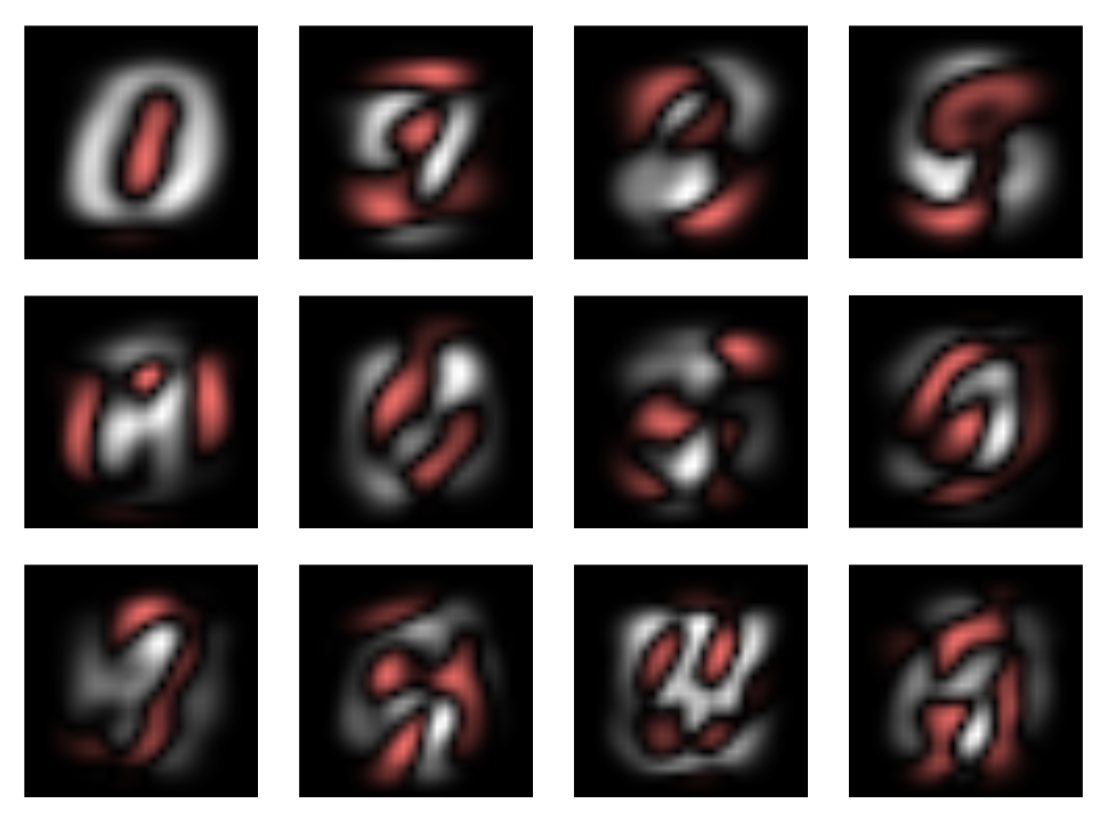
\includegraphics[width=0.7\textwidth]{2-mpca-MNIST-components.png}
  \caption{Above are the first 12 components produced by MPCA over the
    MNIST hand-written digit classification data set. The original
    MNIST data is in strictly black and white, these images are
    normalized to unit 2-norm for visualization purposes. The red
    coloring indicates large magnitude negative values, black is
    neutral, and white is large positive values. Notice the
    resemblance of these components to natural digits.}
  \label{fig:mnist}
  %% {{https://people.cs.vt.edu/tchlux/files/[2018-11-28]_MNIST_12_MPCA_Components.png}}
\end{figure}

\begin{figure}
  \centering
  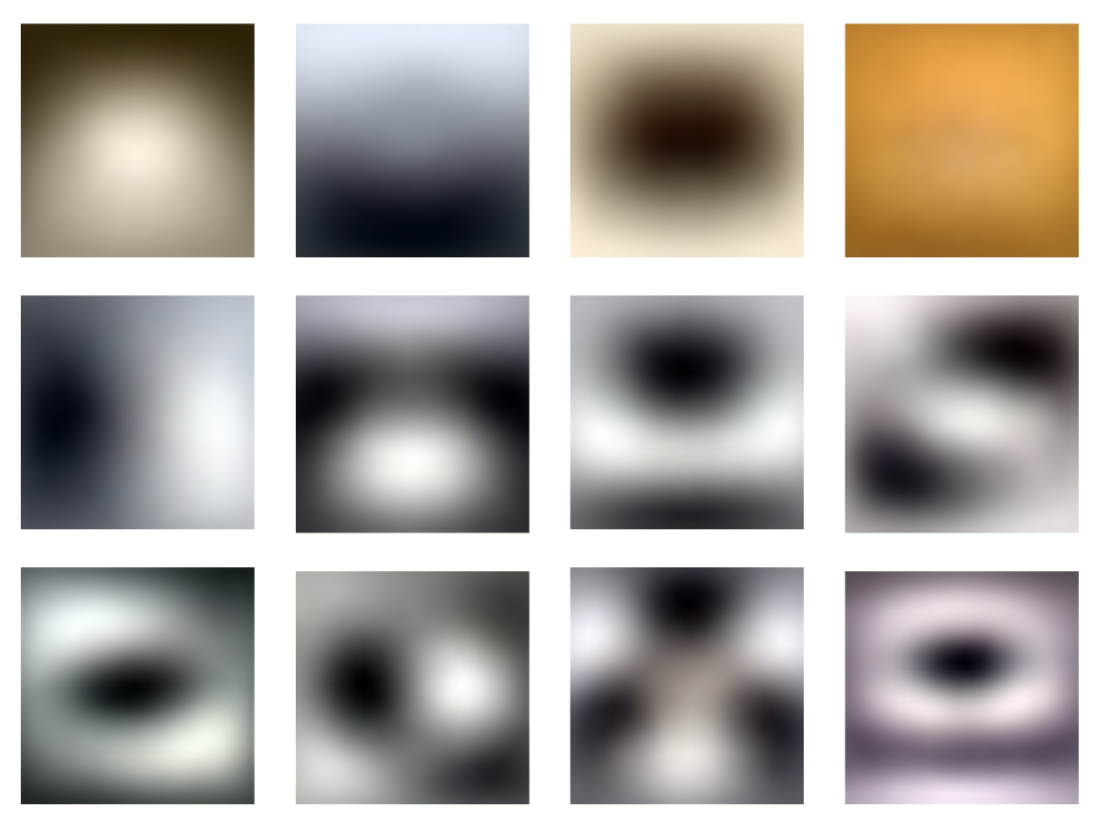
\includegraphics[width=0.7\textwidth]{2-mpca-CIFAR10-components.png}
  \caption{Above are the first 12 components produced by MPCA over the
    CIFAR10 general image classification data set. These images are
    normalized to unit 2-norm before visualization. Notice that the
    components strongly resemble the early terms in a Fourier
    decomposition, suggesting that low frequency spatial oscillations
    contain the most information in images, followed by more varied
    spatial patterns.}
  \label{fig:cifar10}
  %% {{https://people.cs.vt.edu/tchlux/files/[2018-11-28]_CIFAR10_12_MPCA_Components.png}}
\end{figure}


The first 12 components produced by MPCA for the image classification
problems can be seen in Figures \ref{fig:mnist} and
\ref{fig:cifar10}. Notice how the first components are drastically
different even though both are computer vision classification tasks.
This is expected, because recognizing the differences between
handwritten digits and generic objects (with 3-dimensional
orientations) are drastically different problems.

\begin{figure}
  \centering
  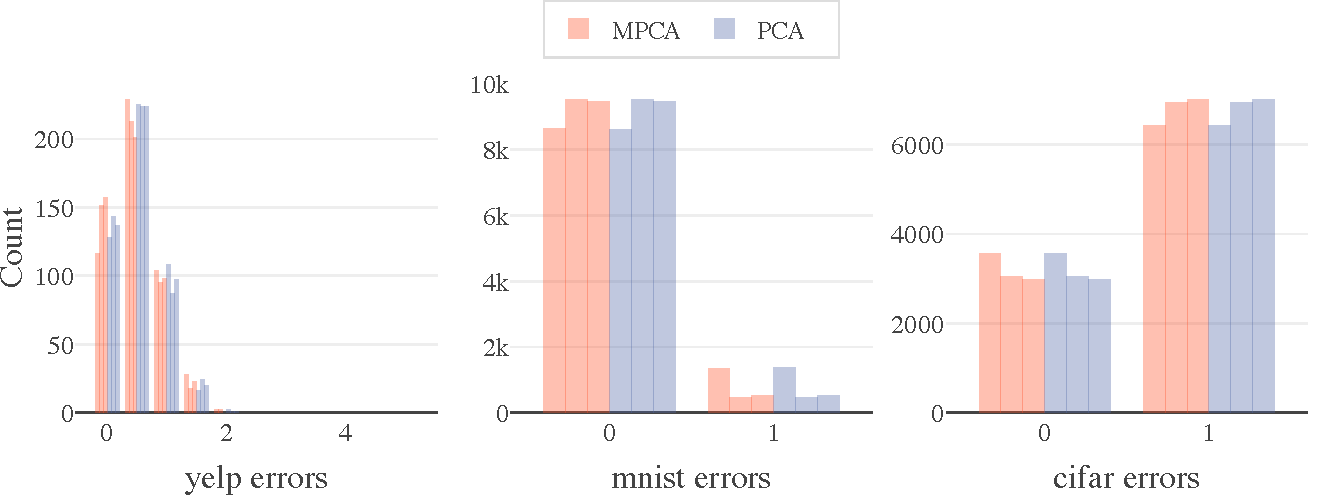
\includegraphics[width=0.9\textwidth]{3-prediction-errors.pdf}
  \caption{The prediction errors of KNN are computed via 4-fold cross
    validation. From left to right, the three bars within each group
    show the performance of KNN with $\{1/100$, $1/10$, $1/3\}$ of all
    features respectively. In general, MPCA and PCA perform similarly
    for all three prediction tasks.}
  \label{fig:errors}
  %% {{https://people.cs.vt.edu/tchlux/files/[2018-11-28]_tgds_errors_hist.html}}
\end{figure}


The prediction errors with varying amounts of dimension reduction by
MPCA and PCA are presented in Figure \ref{fig:errors}. The results
show that common real approximation problems seem to have data
variance that aligns well with the underlying phenomenon being
modeled. This result is somewhat expected, as data sets are often
collected in a way that assumes each piece of information is
specifically relevant to the underlying phenomenon being approximated.

MPCA is used with varying levels of dimension reduction to improve KNN
predictions in Table \ref{tab:mpca-results}. For each approximation
problem, a different amount of reduction produces the best
approximation accuracy. The Yelp data requires the smallest subspace,
MNIST is near the middle, and the CIFAR10 data requires the largest
subspace that is not the raw images.

Finally, results combining all algorithms, data sets, and both PCA and
MPCA are presented in Table \ref{tab:all-results}. Notice that the
empirical results demonstrate that MPCA is not guaranteed to be the
best reduction technique even for strictly distance based prediction
techniques. On the \textit{Yelp} data, PCA still produces better
results for 10-nearest neighbors. It is suspected that the worse
performance of MPCA is due to the reduction on $Z$ and the increased
variability introduced by the random sampling and metric scaling.

These results should not be considered exhaustive, nor should these
results devalue MPCA accordingly. In almost all cases the differences
between the best PCA and MPCA predictors are less than $1\%.$ Aside
from performing similarly, MPCA has the added benefit of accommodating
less careful data collection procedures.


\begin{table}
  \centering
  \renewcommand{\arraystretch}{1.5}
  \begin{tabular}{c c c c c}
    \hline
    \textbf{Data Name} & \textbf{Raw data}
      & \multiline{\textbf{1/3 MPCA}\\[-3mm]\textbf{components}}
      & \multiline{\textbf{1/10 MPCA}\\[-3mm] \textbf{components}}
      & \multiline{\textbf{1/100 MPCA}\\[-3mm] \textbf{components}} \\
    \hline \hline
    \multiline{\textit{Yelp}\\[-3mm]64 dim}
      & 0.493 (stars) & \underline{0.493 (stars)} & 0.496 (stars) & 0.530 (stars) \\
    \multiline{\textit{MNIST}\\[-3mm]784 dim}
      & 5.29\% & 5.26\% & \underline{4.63\%} & 13.43\% \\
    \multiline{\textit{CIFAR10}\\[-3mm]3072 dim}
      & 70.99\% & 70.23\% & 69.46\% & \underline{62.46\%} \\
    \hline
  \end{tabular}
  \vspace{5mm}
  \caption{This table shows the prediction accuracy of a KNN model
    when provided the raw data, and varying size subspaces from MPCA
    for the three real approximation problems. In each problem, the
    optimal size subspace varies. For Yelp, the smallest size subspace
    is best, while for CIFAR10, the largest subspace is best.}
  \label{tab:mpca-results}
\end{table}

\section{Discussion}
\label{sec:discussion}

The error results for reduced-dimension problems using PCA and Metric
PCA (MPCA) are remarkably similar. In almost all cases the MPCA
reduction causes an improvement in prediction accuracy for nearest
neighbor predictions, though the improvement is small. Although an
analytic example demonstrates the potentially large difference between
MPCA and PCA, in practice the two appear to often be nearly
equivalent. One could speculate that this is a contrived phenomenon,
the only data that is kept in curated sets is data that represents a
phenomenon of interest. MPCA is constructed to disregard data that is
not useful, but for the data sets chosen in this work the underlying
data is already distributed according to the functions being modeled.

\begin{table}
  \centering
  \renewcommand{\arraystretch}{1.2}
  \begin{tabular}{c c c c c}
    \hline
    \textbf{Data Set} & \textbf{Approximator}
      & \multiline{\textbf{Reduction}\\[-1mm]\textbf{Technique}}
      & \multiline{\textbf{Reduced}\\[-1mm]\textbf{Dimension}}
      & \multiline{\textbf{Lowest}\\[-1mm]\textbf{Mean}\\[-1mm]\textbf{Error}} \\
    \hline \hline
    \multirow{5}{*}{\textit{Yelp}}
    & Delaunay & PCA & 21 & 0.512 \\
    & KNN (1) & MPCA & 6 & 0.610 \\
    & KNN (10) & PCA & 6 & \underline{0.493} \\
    & LSHEP & raw & 63 & 0.678 \\
    & MLPRegressor & PCA & 1 & 0.515 \\
    \hline
    \multirow{5}{*}{\textit{MNIST}}
    & Delaunay & PCA & 8 & 0.132 \\
    & KNN (1) & MPCA & 78 & \underline{0.046} \\
    & KNN (10) & MPCA & 78 & 0.051 \\
    & LSHEP & PCA & 8 & 0.139 \\
    & MLPRegressor & PCA & 261 & 0.133 \\
    \hline
    \multirow{5}{*}{\textit{CIFAR10}}
    & Delaunay & PCA & 31 & 0.369 \\
    & KNN (1) & MPCA & 31 & 0.319 \\
    & KNN (10) & MPCA & 31 & 0.357 \\
    & LSHEP & PCA & 31 & 0.350 \\
    & MLPRegressor & raw & 3072 & \underline{0.103} \\
    \hline
  \end{tabular}
  \vspace{5mm}
  \caption{In this expanded set of results, the optimal reduction
    technique and subspace size is presented for each algorithm and
    for each real approximation problem. Notice that MPCA is not the
    most common \textit{best} reduction technique, which is
    counterintuitive. This suggests that the data provided for each
    approximation problem is in fact representative of the underlying
    phenomenon being modeled. It also suggests that the noise
    introduced in randomly sampling pairwise vectors for MPCA may
    inhibit its performance on approximation problems that are
    well-represented by available data.}
  \label{tab:all-results}
\end{table}

\section{Conclusion}
\label{sec:conclusion}

The proposed technique, Metric PCA, demonstrates strong potential as a
dimension reduction strategy for approximation problems. Analytically,
Metric PCA is not susceptible to adverse data conditions that may
cause PCA to disregard important dimensions for
approximation. Empirically, the results obtained by MPCA and PCA are
quite similar, suggesting that many curated data sets have the
property that data variance corresponds closely to variance
in the underlying function. Analytic and empirical results combined
demonstrate the effectiveness of MPCA as a robust dimension reduction
strategy for approximation.


%% \begin{figure}[htb]
%%   \centering
%%   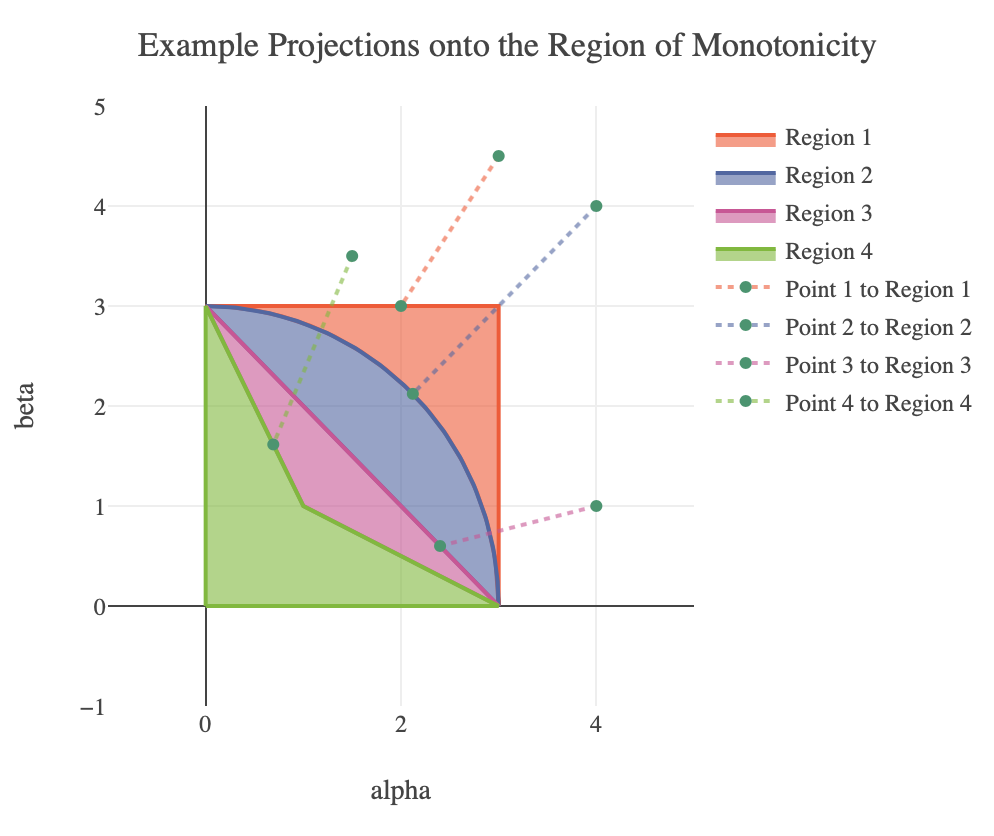
\includegraphics[width=0.50\textwidth]{demo_projection}
%%   \caption{These are the projection mechanisms that make a cubic polynomial piece monotone.}\label{fig:projection}
%% \end{figure}



% Please don't change the bibliographystyle style
\bibliographystyle{scsproc}
% AUTHOR: Include your bib file here
\bibliography{paper}


\section*{Author Biographies}

\textbf{\uppercase{THOMAS C. H. LUX}} is a Ph.D. candidate in computer
science at Virginia Polytechnic Institute and State University
(VPI\&SU) studying under Dr. Layne Watson. His research interests
include computational science, approximation theory, optimization, and
artificial intelligence. His email address is \email{tchlux@vt.edu}.

\textbf{\uppercase{Tyler H. Chang}} is a Ph.D. candidate at VPI\&SU
studying computer science under Dr. Layne Watson.


\end{document}
